\section{Mô hình phía phát}

Hình \ref{fig:Transmitter} biểu diễn OFDMA-MU-MIMO trong tiêu chuẩn 802.11ax và hệ thống OFDMA-IDMA được đề xuất. Có thể thấy rằng mô hình đề xuất trong Hình \ref{fig:Proposed_OFDMA-IDMA} có khối tương tự như OFDMA-MU-MIMO trong Hình \ref{fig:Old-OFDMA-MU-MIMO}. Tuy nhiên, trong mô hình đề xuất, thay vì thực hiện quá trình phân luồng không gian, các STA chỉ thực hiện quá trình trải và xen kẽ.
Trong báo cáo này, mã xen kẽ được sử dụng hiệu quả hơn IDMA thông thường bằng cách kết hợp với OFDMA; các mã này được sử dụng lại trong các RU khác nhau, nhằm tăng số lượng STA trong khi vẫn không làm tăng số lượng mã bộ chèn.
Ngoài ra, để tương thích với LDPC trong chuẩn 802.11ax khi thêm khối bộ mã hóa IDMA vào quy trình, các tham số $N_{pld,u}$ và $N_{avbits,u}$ trong phương trình (27-29) và phương trình(27-80) trong \cite{IEEEStd} được thay thế bằng \eqref{eq:14} và \eqref{eq:15}
% \vspace{-0.5em}
\begin{equation}
    \begin{split}
        N_{pld,u} = &{\text{SF}}^{-1}((N_{\text{SYM,init}}-m_{\text{STBC}} \mathord{\times} \text{SF}) \mathord{\times} N_{\text{DBPS},u} \\
        &+ m_{\text{STBC}} \mathord{\times} N_{\text{DBPS,last,init},u}), 
    \end{split}
    \label{eq:14}
\end{equation}

\begin{equation}
    \begin{split}
        N_{avbits,u} = &{\text{SF}}^{-1}((N_{\text{SYM,init}}-m_{\text{STBC}} \mathord{\times} \text{SF}) \mathord{\times} N_{\text{CBPS},u} \\
        &+ m_{\text{STBC}} \mathord{\times} N_{\text{CBPS,last,init},u}),
    \end{split}
    \label{eq:15}
\end{equation}
với $N_{\text{DBPS,last,init},u}$, $N_\text{SYM,init}$, $m_{\text{STBC}}$, $N_{\text{DBPS}, u}$, $N_{\text{CBPS},u}$, $N_{\text{CBPS,last,init},u}$ có cùng định nghĩa trong \cite{IEEEStd} và SF là hệ số trải phổ sử dụng trong IDMA.
\begin{figure}
    \centering
    \begin{subfigure}{0.49\linewidth}
        \centering
        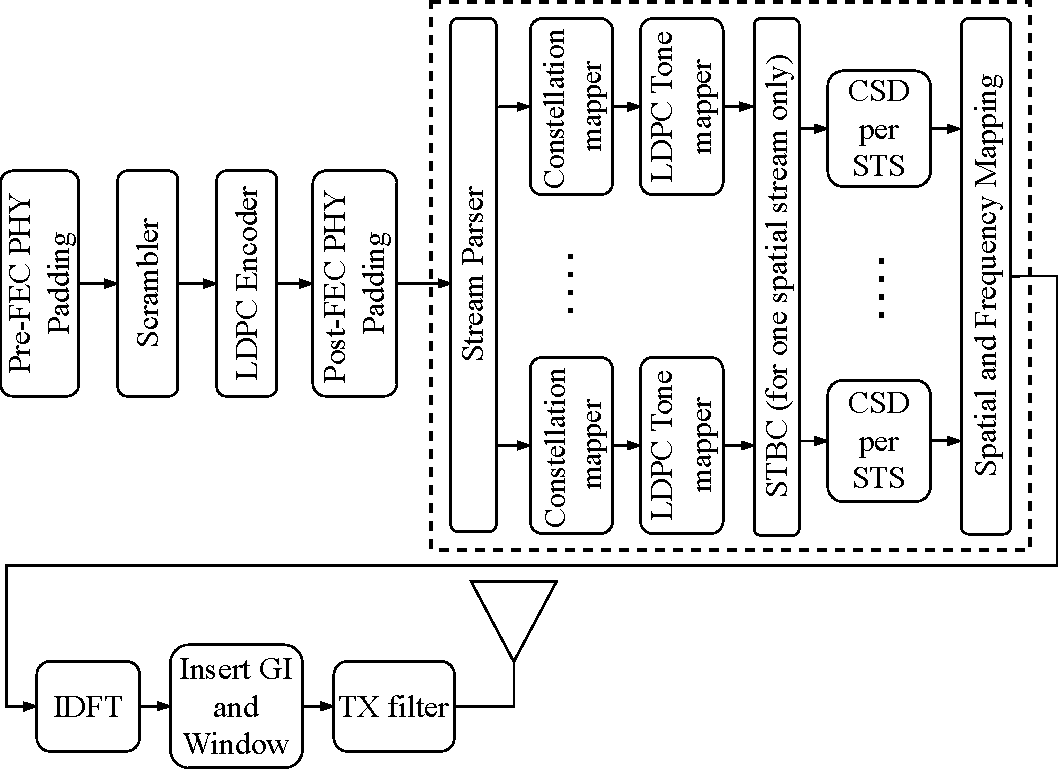
\includegraphics[width=1.2\linewidth, angle = -90]{figure/chap3/MU-MIMOTx_k2opt.pdf}
        \caption{OFDMA-MU-MIMO 802.11ax.}
    \label{fig:Old-OFDMA-MU-MIMO}
    \end{subfigure}
    \vspace{1em}
    %==============
    \begin{subfigure}{0.49\linewidth}
        \centering
        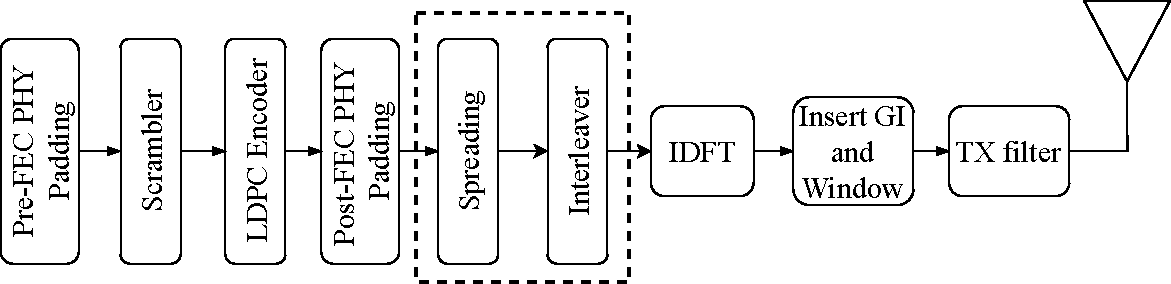
\includegraphics[width=\linewidth, angle = -90]{figure/chap3/IDMA_Tx_Rx_structure-Trang-4_k2opt.pdf}
        \caption{OFDMA-IDMA đề xuất dựa trên 802.11ax.}
    \label{fig:Proposed_OFDMA-IDMA}
    \end{subfigure}

    \caption{Kiến trúc đường lên với mã hóa LDPC.}
    % \vspace{-1em}
    \label{fig:Transmitter}        
\end{figure}
\section{Mô hình phía thu}

Để xác thực tính khả thi của hệ thống được đề xuất trong môi trường WLAN, chúng tôi trình bày cách triển khai bộ thu được mô tả trong Hình \ref{fig:OFDMA-IDMARx}. Kiến trúc bộ thu phản chiếu bộ thu 802.11 tiêu chuẩn cho đến giai đoạn ESE, nơi quá trình xử lý IDMA bắt đầu. Bài viết này sử dụng giải mã IDMA kết hợp với MRC như trong Hình \ref{fig:IDMASystem}. Việc lựa chọn số lần lặp trong giải mã IDMA là rất quan trọng, ảnh hưởng đến cả hiệu suất và độ trễ. Sau mỗi lần lặp, các giá trị thống kê về nhiễu và nhiễu được cập nhật cho các phép tính tiếp theo, cải thiện độ chính xác với số lần lặp tăng lên. Tuy nhiên, số lần lặp nhiều hơn cũng có nghĩa là độ trễ tính toán cao hơn. Để đáp ứng mục tiêu độ trễ 10 $\mu s$ phù hợp với tiêu chuẩn 802.11, chúng tôi áp dụng bốn lần lặp, như được xác định trong \cite{UL-OFDM-IDMA} với SF là 2 trong thiết lập của chúng tôi.

\begin{figure}[H]
    \centering
        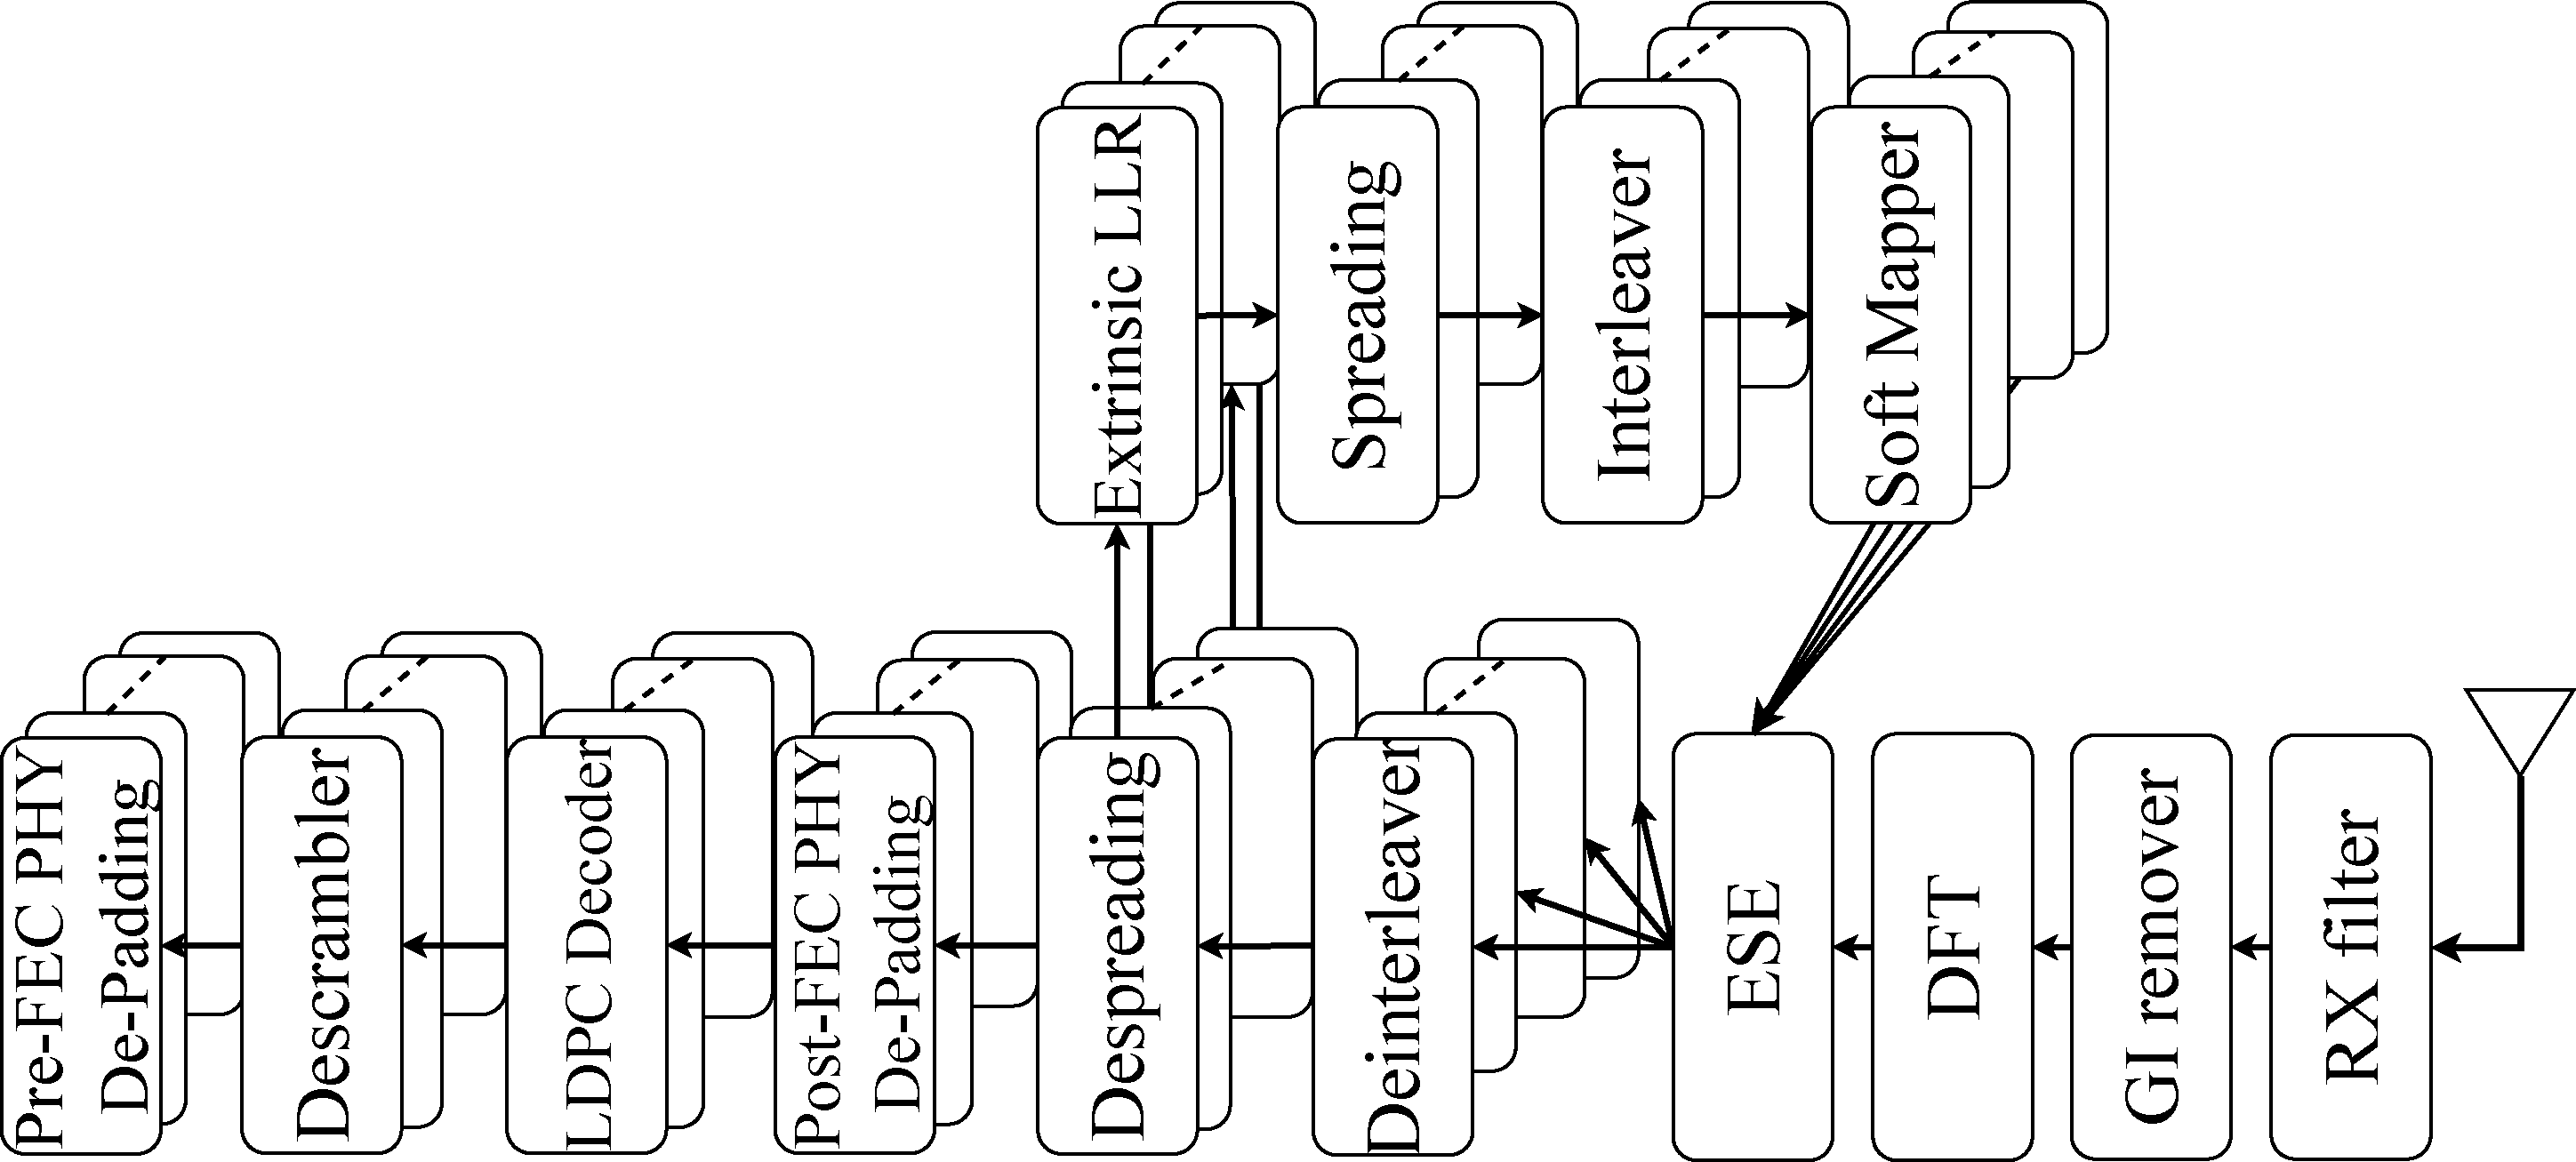
\includegraphics[width=0.75\linewidth]{figure/chap3/Proposed_Receiver.pdf}
    \caption{Proposed receiver architecture.}
    \label{fig:OFDMA-IDMARx}
    % \vspace{-1em}
\end{figure}